\section{Discussion}

\subsection{Wind Does Not Disrupt Overwintering Monarch Butterflies}

Our study provides the first direct empirical test of the disruptive wind hypothesis and finds no support for wind as a primary factor influencing monarch butterfly clustering behavior. Despite the widespread adoption of the 2 m/s wind threshold in conservation practice \autocite{Society2016_WFJMUMAD}, our data reveal no relationship between wind speed and butterfly departures across the full range of observed conditions (0--12 m/s). While our models explain only 5.7\% of variance in butterfly movements, reflecting our focus on testing wind effects rather than comprehensively explaining movement patterns, they had sufficient statistical power to detect environmental signals. This finding challenges assumptions underlying three decades of management guidance.

The absence of wind effects in our data is particularly striking given that observed mean maximum wind speeds (2.2 m/s, SD = 1.4) frequently exceeded the proposed threshold. If the disruptive wind hypothesis were valid, we should have observed a clear signal: substantial reductions in butterfly abundance, as predicted by the disruptive wind hypothesis. Instead, we observed no change, small changes, or even positive changes in butterfly abundance at wind speeds six times the proposed disruption threshold. 

Importantly, our power analysis demonstrated 87.5\% power to detect moderate effect sizes (0.15 standard deviations) and 98.5\% power for larger effects (0.20 standard deviations), while wind appeared in only one of the top five models (M24). In that model wind showed little evidence of an effect (p = 0.218) and resulted in substantially poorer model performance compared to the best model (ΔAIC = 6.2, capturing only 4\% of model weight). This weak wind signal, combined with our high statistical power, allows us to rule out all but very small wind effects. Given that the disruptive wind hypothesis predicts conspicious reduction in abundance above threshold wind speeds, a substantial effect by any measure, our failure to detect such patterns provides strong evidence against the hypothesis rather than merely absence of evidence.

The methodological validity of our approach is confirmed by the strong signals detected for other environmental variables. Had our counting method or analytical framework been flawed, we would not have captured the pronounced effects of direct sunlight (F = 19.36, p < 0.001) or the complex diurnal patterns (F = 8.90, p < 0.001) that emerged from the same dataset.

\subsection{Alternative Drivers of Monarch Movement}

While our study was designed specifically to test the wind hypothesis, our results suggest that thermoregulation, light exposure, and diurnal rhythms play more important roles than wind in driving short-term movements at overwintering sites.

\subsubsection{Direct Sunlight as the Strongest Predictor}

Direct sunlight exposure emerged as the strongest environmental predictor of reductions in cluster abundance in our study (F = 19.36, p < 0.001). Butterflies exposed to direct sunlight at the beginning of an observation interval showed the largest decreases in abundance, suggesting that solar radiation rapidly increases butterfly body temperatures well above ambient conditions. This finding aligns with \citeauthor{Masters1988_ACNENTPT}'s work showing that monarchs in direct sunlight can elevate their body temperature above ambient conditions within minutes. This rapid warming capability could readily explain why direct sunlight exposure is such a strong predictor of decreased abundance at clusters.

The relationship between sunlight and departure represents a key component of the thermoregulatory equation. Monarchs have evolved to efficiently absorb solar radiation, an adaptation that enables flight at temperatures below what would otherwise be physiologically possible \autocite{Masters1988_ACNENTPT}. Yet this same efficiency becomes a liability when clustering. Butterflies cannot avoid absorbing heat when exposed to direct sun, risking overheating and accelerated depletion of their finite lipid reserves through elevated metabolism \autocite{Masters1988_ACNENTPT}. This forces them to abandon energetically favorable clustering positions even when ambient temperatures remain cool. This trade-off between the benefits of clustering and the thermal constraints imposed by solar exposure may fundamentally shape daily movement patterns at overwintering sites.

\subsubsection{Temperature Effects and Their Interpretation}

Ambient temperature showed a subtle but significant relationship with monarch abundance changes (EDF = 3.93, F = 3.23, p = 0.028). The data suggest minimal change below 15°C (the known flight threshold), a slight positive association around 20--21°C, and sharp declines above 25°C consistent with thermoregulatory constraints. Given that available temperatures vary latitudinally across overwintering sites \autocite{Saniee2022_3VN7I68M}, our results from Spring Canyon capture only a portion of the temperature continuum experienced across the entire overwintering range. The temperature effects we observed reflect responses within the specific thermal envelope available at our study latitude. Testing these patterns at sites spanning the full latitudinal gradient would reveal whether monarch responses to temperature are consistent or vary with local thermal regimes.

\subsubsection{Diurnal Activity Patterns}

Time since sunrise revealed distinct diurnal patterns (EDF = 4.90, F = 8.90, p < 0.001), with butterflies departing clusters in the morning and reforming aggregations in the afternoon. This pattern persists even after controlling for temperature and sunlight, aligning with anecdotal observations from overwintering sites throughout California.

\subsection{Study Limitations}

Several limitations warrant consideration. Our data derive from a single season (2023--2024) with typical monarch abundance at two sites. The following season (2024--2025), virtually no clustering monarchs were observed at Vandenberg Space Force Base (23 individuals total) despite monitoring 10 sites. This coincided with the second-lowest overwintering population on record statewide \autocite{xerces_society_western_2025}, preventing temporal replication of our study. Additionally, our counting methodology introduced discretization artifacts that contributed to large confidence intervals for environmental predictors. While we detected strong signals like direct sunlight effects, more subtle relationships require careful interpretation.

Furthermore, our study observed clusters where butterflies maintained direct substrate contact. In historically massive aggregations containing hundreds of thousands of individuals, many butterflies attach only to other butterflies, creating multi-layered formations. If substrate attachment confers greater wind resistance than butterfly-to-butterfly attachment, the disruptive wind hypothesis might apply specifically to these larger aggregations. Future work should examine whether wind responses differ between substrate-attached and butterfly-attached individuals, particularly at sites supporting extreme densities.

\subsection{Management Implications}

Our findings suggest that management strategies prioritizing wind protection warrant reconsideration. The absence of wind effects despite frequent threshold exceedances indicates that usable habitat within existing groves may be larger than currently recognized. Areas previously dismissed due to perceived wind exposure may provide suitable conditions because they offer appropriate light and thermal regimes.

While past management efforts aimed at wind protection may have been based on incomplete understanding, they likely produced beneficial outcomes by increasing tree density. The fundamental recommendation to plant and maintain trees remains sound. Management should prioritize maintaining existing mature trees while establishing future roosting habitat at densities that support healthy, long-lived growth. In addition, as suggested by Saniee and Villablanca (2022), it may become relevant to explore ways in which to manage for thermal attributes, specifically sunlight.

\subsection{Future Research Directions}

Our findings open several important avenues for future research. First, explicit testing of light patterns as predictors of clustering locations could establish whether canopy structure guides habitat selection. The strong effect of direct sunlight (F = 19.36, p < 0.001) combined with the predictability of canopy-created light patterns suggests this may be a primary factor in roost site selection. Previous research also suggests light conditions may play an important role in habitat selection. \autocite{Weiss1991_ESKZGQJV} used hemispherical photography to measure the Indirect Site Factor (ISF), which quantifies percent canopy openness, across sites with different occupancy histories. Permanent overwintering sites clustered within a narrow range of canopy openness (approximately 20\%) with relatively low variance, while transient and unoccupied sites showed progressively greater variability (Figure \ref{fig:weiss_canopy}). This pattern of consistent light conditions at successful sites provides additional context for understanding how canopy structure might influence clustering behavior.

\begin{figure}[h]
    \centering
    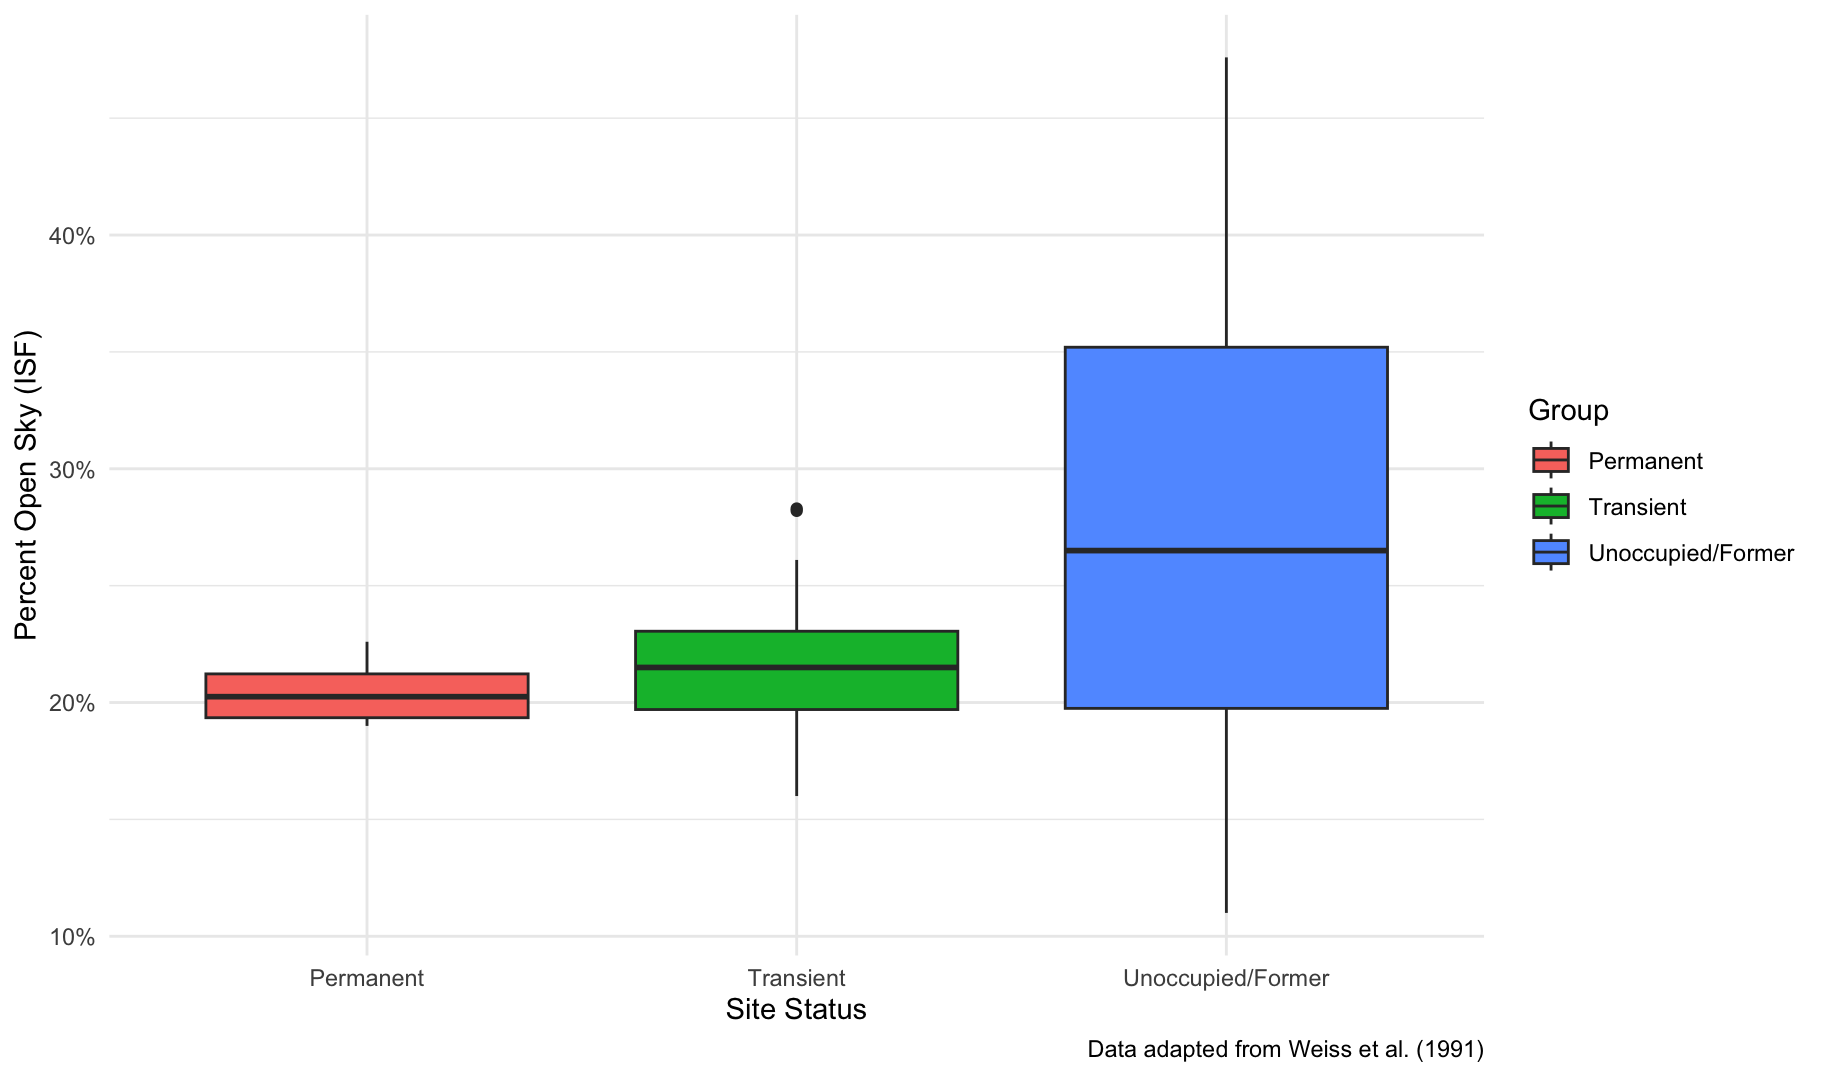
\includegraphics[width=0.8\textwidth]{figures/discussion/weiss_adapted_boxplot.png}
    \caption{Percent canopy openness (Indirect Site Factor) by occupancy status, adapted from Weiss et al. (1991). Permanent overwintering sites exhibit both a specific range of canopy openness (~20\%) and lower variance compared to transient and unoccupied/former sites.}
    \label{fig:weiss_canopy}
\end{figure}

Second, investigation of social dynamics and positive behavioral feedback mechanisms could address unexplained variation in our models. Monarchs may exhibit emergent clustering behaviors where initial settlement increases the probability of others joining, creating self-reinforcing patterns independent of environmental conditions.

Research should also examine whether our findings extend across the broader overwintering range. Testing these patterns at sites with different tree species, latitudes, and in particular population densities would strengthen conclusions about the generality of wind effects, or their absence.

\subsection{Conclusions}

Wind did not disrupt monarch clusters even at speeds far exceeding presumptive thresholds. Instead, butterflies responded primarily to thermal conditions, including light exposure and ambient temperature, and to diurnal rhythms. These findings challenge current assumptions about overwintering habitat requirements and suggest that management priorities should be reevaluated. While our study represents one season at two sites, the absence of wind effects despite adequate statistical power raises important questions regarding decades of conservation guidelines. As monarch populations face continued threats, evidence-based management becomes increasingly critical for conserving the overwintering sites essential for this iconic species.